\documentclass{VUMIFPSkursinis}
\usepackage{algorithmicx}
\usepackage{algorithm}
\usepackage{algpseudocode}
\usepackage{amsfonts}
\usepackage{amsmath}
\usepackage{bm}
\usepackage{caption}
\usepackage{color}
\usepackage{float}
\usepackage{graphicx}
\usepackage{listings}
\usepackage{subfig}
\usepackage{wrapfig}

% Titulinio aprašas
\university{Vilniaus universitetas}
\faculty{Matematikos ir informatikos fakultetas}
% \institute{Informatikos institutas}  % Užkomentavus šią eilutę - institutas neįtraukiamas į titulinį
\department{Programų sistemų studijų programa}
\papertype{Kursinis darbas}
\title{Paukščių ant pastatų aptikimas ir atbaidymas naudojant konvoliucinius neuroninius tinklus ir lazerius}
\titleineng{Detection and deterrence of birds on buildings using convolutional neural networks and lasers}
\status{4 kurso 1 grupės studentas}
\author{Tautvilis Savickas}
\supervisor{Prof. Dr. Aistis Raudys}
\date{Vilnius – \the\year}

% Nustatymai
  % Pakeisti teksto šriftą į Palemonas (turi būti įdiegtas sistemoje)
\bibliography{bibliografija}

\begin{document}
\maketitle

\tableofcontents

\sectionnonum{Įvadas}

Paukščių būriai sukelia daug žalos ūkiams bei miestams. Ūkininkai patyria didelę ekonominę žalą, kadangi paukščiai yra sudėtingi ir  mobilus kenkėjai - jie sunaikiną derlių \cite{refId0} ir platina ligas, kaip paukščių gripas. Miestuose paplitę paukščiai, kaip miesto balandžiai (Columba livia domestica) ar tikrieji varnėnai (Sturnus), daro didelę žalą savo išmatomis. Kadangi jie peri ant miesto pastatų, jų išmatos kaupiasi ir nėra dažnai valomos \ref{img:bird_poop} pav., todėl tampą skirtingų ligų šaltiniu. Jungtinėse Amerikos Valstijose invaziniai paukščiai sukėlė 1,1 milijardo JAV dolerių žalos \cite{article}. Taip pat balandžių išmatos yra labai rūgštingos ir gali padaryti žalą metalams bei mūriniams objektams, pavyzdžiui: mašinos, pastatai, paminklai. \cite{ahmed2021effect, shrestha2022conservation}.

\begin{figure}[H]
    \centering
    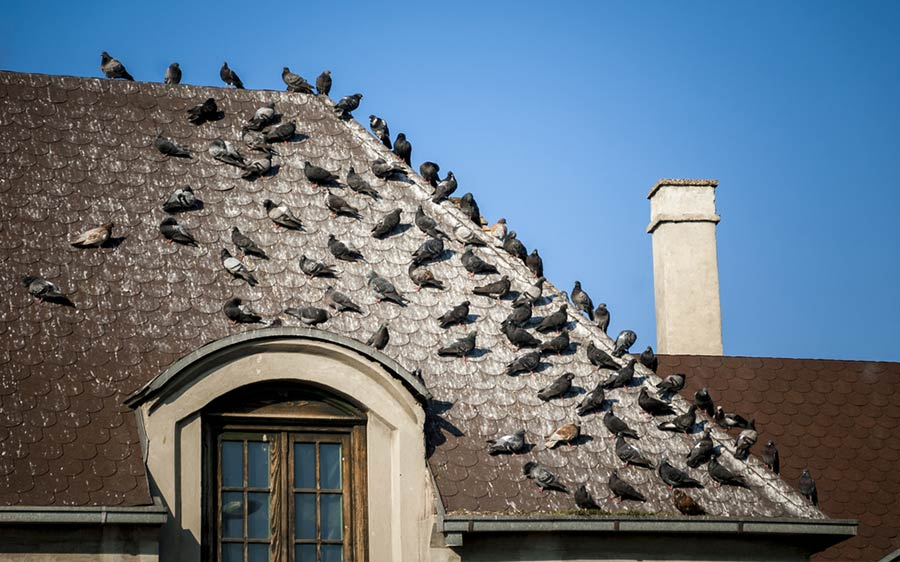
\includegraphics[scale=0.5]{img/bird_poop_on_roof.png}
    \caption{Balandžių pulko padaryta žala stogui. Šaltinis: \href{https://shamrockroofer.com/keep-birds-from-nesting-on-the-roof-with-these-5-tips/}{https://shamrockroofer.com/keep-birds-from-nesting-on-the-roof-with-these-5-tips/}}
    \label{img:bird_poop}
\end{figure}


Vienas iš gausiai paplitusių būdų atbaidyti paukščius, kuris nekenkia paukščiams ir yra paprastas naudoti yra lazeriai. 1970-aisiais metais buvo pradėtas naudotas, kad apsaugotu lėktuvus nuo susidūrimo su paukščiais. Vėliau, lazeriai pradėti naudoti ir plačiau: ūkiuose, naftos platformose. JAV kukurūzų ūkininku laukuose be lazerinių atbaidymo prietaisų žala svyravo tarp 40 \% ir 100 \%, tačiau naudojant lazerius - sumažėjo iki 5 \% \cite{brown2017laser}.


Šio darbo tikslas yra sukurti sprendimą, kuris gebėtų atpažinti paukščius esančius ant stogų ir juos nubaidytų naudojant lazerį. Darbas pradedamas nuo trumpos alternatyvų analizės. Toliau darbe rašoma apie duomenų rinkinio kūrimą, palyginami trys YOLO objektų aptikimo realiu laiku modelių versijos. Taip pat siūlomas atbaidymo sistemos dizainas. Darbo rezultatas yra pilno sprendimo dizainas aptikti ir atbaidyti paukščius, kurį būtų galima įgyvendinti.


\section{Apsisaugojimo nuo paukščių alternatyvos}
Alternatyvių sprendimų rinkoje yra keletas - mechaniniai, akustiniai, natūralus ir optiniai. Šiame skyriuje paanalizuosime sprendimus iš kiekvienos kategorijos \ref{img:deterrents} pav.

\begin{figure}[H]
    \centering
    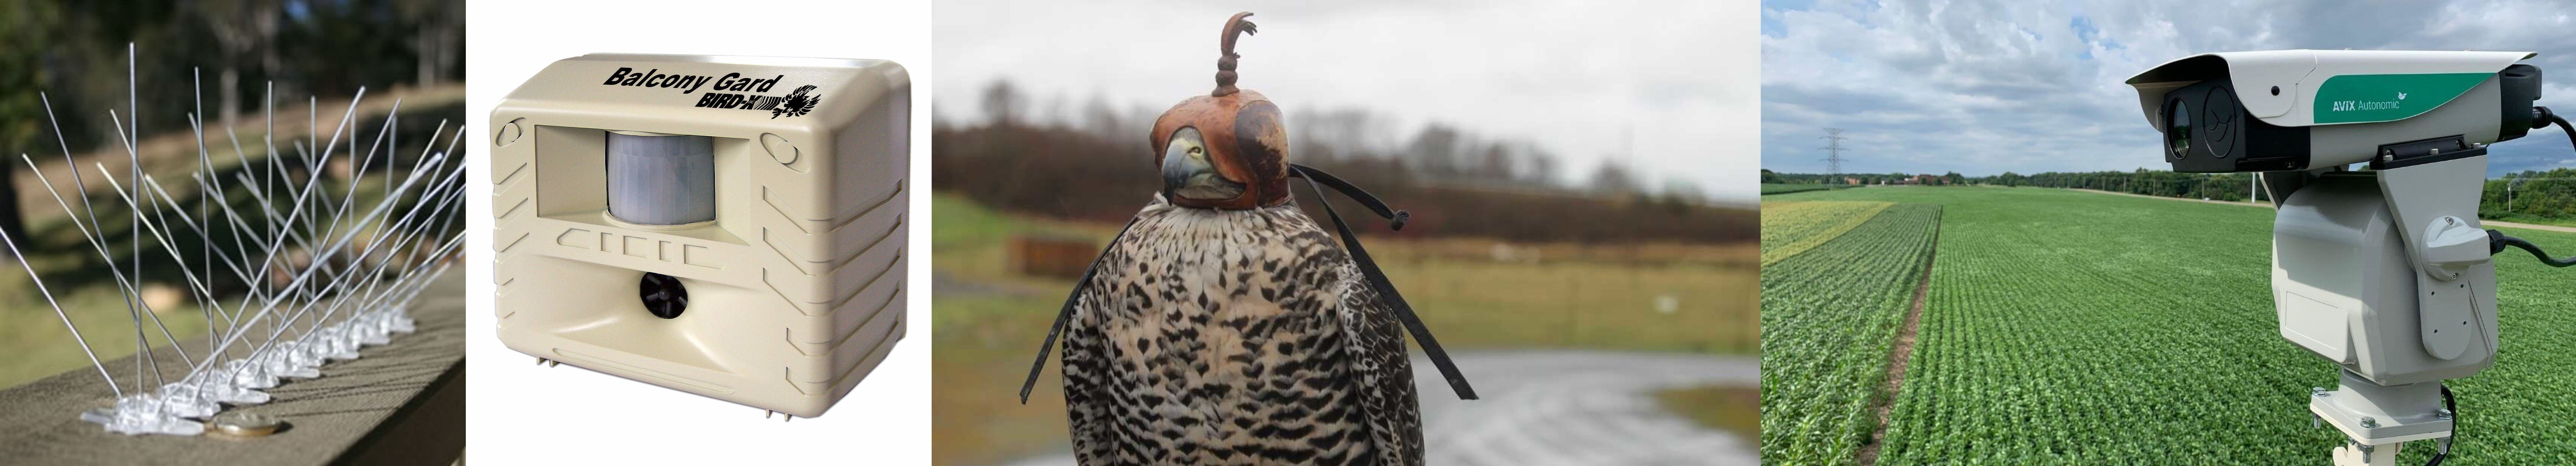
\includegraphics[width=0.8\textwidth]{img/deterrents.jpg}
    \caption{Paukščių atbaidymo sprendimai.}
    \label{img:deterrents}
\end{figure}

\subsection{Mechaninis būdas}
Vienas iš populiariausių būdų apsisaugoti nuo paukščių yra spygliai. Jie būna konstruojami tose vietose, kur dažniausiai yra pastebimi paukščiai. Dažnai tai būna pastato stogai, tvoros ar lietvamzdžiai. Šis būdas yra plačiai paplitęs, kadangi tai efektyviai apsaugo turtą nuo paukščių sukeliamos žalos. Tačiau tai dažnai reikalauja daug finansų, gali greitai suirti, jei nebus tinkamai prižiūrimi. Taip pat sukelia žalą paukščiams.

Dar yra sukurtas vienas naujas ir modernus būdas atgrasinti paukščius - bepiločiai orlaiviai arba dronai \cite{goel2017detection}. Šis sprendimas dažniausiai susideda iš sumontuojamos kameros, kuri stebi tam tikrą apibrėžtą vietą. Kai kamera užfiksuoją paukščius, automatinė sistema aktyvuoja dronus ir jie skrendą į vietą, kur buvo aptikti paukščiai. Šį sprendimą labai riboja bepiločių orlaivių įstatymai, skrydžio laikas ir gamtos stichijos, kaip vėjas ir lietus.

\subsection{Akustinis būdas}
Labiausiai populiarus akustinis būdas yra garsiniai prietaisai. Tai yra garso kolonėlė, kuri skleidžia garso bangas didesnes tam tikruose dažniuose, kuris nėra malonus paukščiams \cite{beason2004can}. Šis aukšto dažnio garsas nemalonus paukščiams, dėl to jie vengia vietų, kur šis garsas skleidžiamas. Šie sprendimai būna montuojami kartu su judesio davikliais, kad galėtų pradėti leisti garsą, kai paukštis būna daviklio ribose. Toks atbaidymo būdas yra labai ribotas, kadangi jis veikia tik nedideliu atstumu, skirtingi dažniai veikia tik tam tikrus paukščius ir pats garsas yra girdimas žmonių, todėl sukelia nepatogumų naudojant vietose, kur lankosi žmonės.

\subsection{Natūralus būdas}
Natūralūs būdai paukščių baidymui yra plėšrūnai. Dažniausiai tai būna dresiruoti sakalai \cite{steensma2016bird}. Kadangi sakalai medžioja smulkius paukščius, šis natūralus būdas yra labai veiksmingas, tačiau šis metodas reikalauja daug laiko ir išlaidų.

\subsection{Optinis būdas}
Ganėtinai senas būdas yra pasitelkiant lazerius. Kadangi lazerio šviesą paukščiai mato kaip kietą kūną, jiems atrodo, kad tai yra artėjanti grėsmė. Tik pradėjus naudoti šią technologiją, buvo naudojami rankiniai lazeriai, tačiau tai padidindavo išlaidas, kadangi reikalingas asmuo, kuris stebėtų ir šviestų su lazeriu. Tačiau pastaraisiais metais yra atsiradę automatiniai sprendimai, kurie stebi nurodytą plotą ir pradeda šviesti, kai jame pastebi paukštį \cite{szentpeteri2018bird}.  Šis būdas atbaidyti paukščius yra efektyvus, lengvai paruošiamas ir nekelia žalos paukščiams, bet jo pradinė kainą yra gana didelė.



\section{Duomenų rinkinys}
Giliojo mokymo objektų aptikimo metodai reikalauja anotuotų duomenų rinkinių, tai yra - kiekviena nuotrauka turi turėti žymes su aptiktu objektu ir jo stačiakampiu. Šis rinkinys buvo sudarytas, kadangi nebuvo rasta alternatyvų, kurie turėtų paukščių nuotraukas padarytas iš tolimesnio atstumo ir paukščiai būtų miesto erdvėse. Šiam darbui buvo sukurtas duomenų rinkinys, kuriame yra 277 anotuotos nuotraukos. Po duomenų augmentacijos, rinkinį sudarė 665 nuotraukos. Iš jų 88 \% mokymosi nuotraukos, 8 \% validavimo ir 4 \% testavimo.

\subsection{Nuotraukų ir anotacijų surinkimas}
Nuotraukoms surinkti buvo naudojama pakoreguota „BBID“ (Bulk Bing Image Downloader) \cite{bbid2014} programa. Ši programa priima raktažodžius ir parsiunčia nurodyta kiekį nuotraukų iš „bing“ paieškos sistemos. Tikrinant šią programinę įrangą buvo pastebėta, kad pareikalavus didesnio kiekio nuotraukų, dalis jų būdavo netikslios, pavyzdys pateiktas \ref{img:monkey_on_roof} pav. Šiai problema išspręsti buvo nuspręsta panaudoti „Amazon Rekognition“ \cite{rekognition} - tai internetinė programa kuri, įkėlus į ją nuotrauką, grąžina visus aptiktus objektus ir jų koordinates nuotraukoje. „BBID“ programinis kodas buvo pakoreguotas, kad kai yra parsiunčiama nuotrauka, ji būtų pateikiama „Amazon Rekognition“ per jų naudojamą internetinę aplikacijų programavimo sąsaja (angl. \emph{Application Programming Interface, API}), tada būtų patikrinimą ar nuotraukoje yra paukštis ir jeigu taip, ši nuotrauka ir aptikto paukščio koordinatės būna išsaugomos. Šio principo veikimo schema pavaizduota \ref{img:bbid} pav. Kadangi anotacijos buvo grąžinamos iš „Amazon Rekognition“, nereikėjo to padaryti rankomis naudojant nemokamą internetinį įrankį „CVAT” \cite{CVAT_ai_Corporation_Computer_Vision_Annotation_2022}. Taip naudojant „Amazon Rekognition“ buvo išspręstos dvi duomenų rinkinio sudarymo užduotys: nuotraukų surinkimas ir jų anotavimas.


\begin{figure}[H]
    \centering
    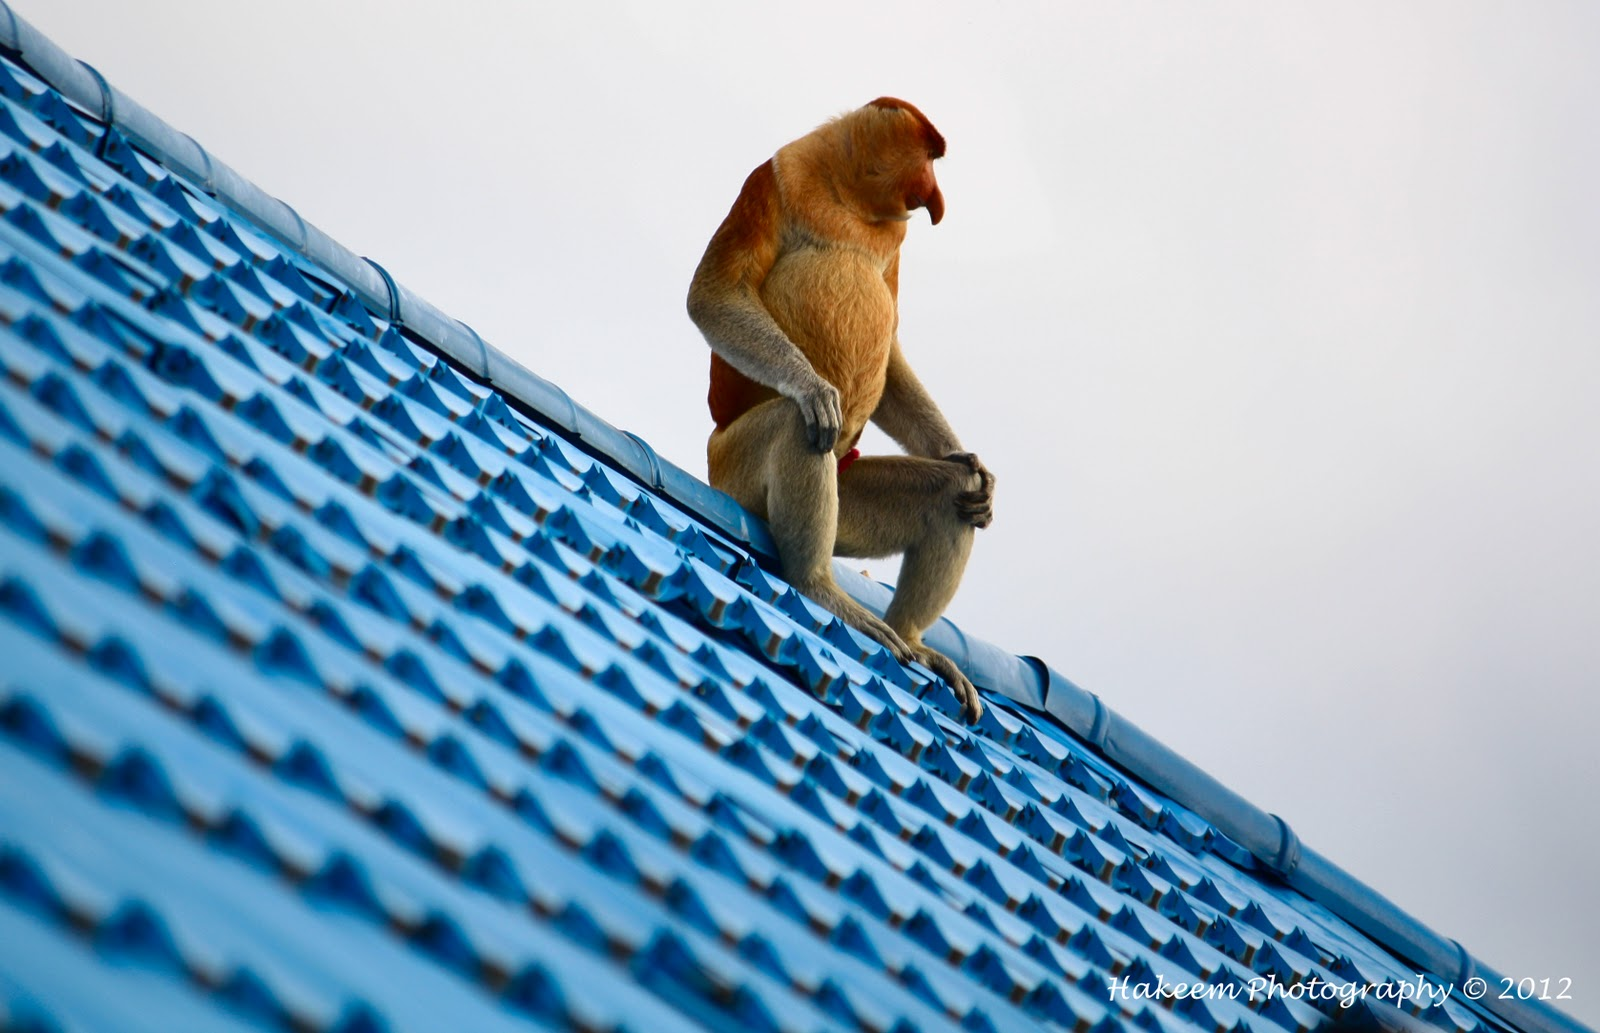
\includegraphics[scale=0.2]{img/sitting+on+the+roof.jpg}
    \caption{„BBID“ programai pateikus raktažodį „\emph{birds on a house}“ grąžinta nuotrauka. Šaltinis: \href{https://photoku-photokita.blogspot.com/2012/01/sitting-on-roof.html}{https://photoku-photokita.blogspot.com/2012/01/sitting-on-roof.html}}
    \label{img:monkey_on_roof}
\end{figure}

\begin{figure}[H]
    \centering
    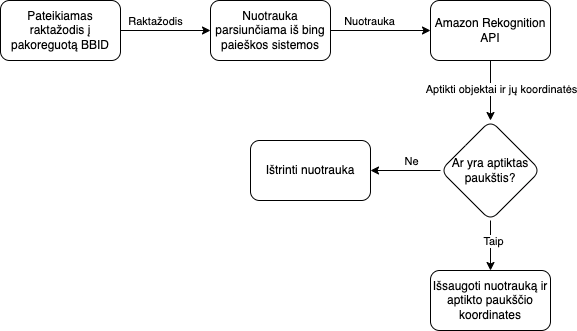
\includegraphics[scale=0.6]{img/bbid_diagrama.png}
    \caption{Nuotraukų atrinkimo schema.}
    \label{img:bbid}
\end{figure}

\subsection{Duomenų rinkinio formavimas}
Formuojant duomenų rinkinį buvo naudojama internetinė programa „roboflow“ \cite{roboflow}. „roboflow“ - tai kompiuterinės regos kūrimo karkasas, kuris palengvina duomenų rinkinių ir modelių kūrimą. Šio darbo metu „roboflow“ buvo naudotas pritaikyti nuotraukoms jų anotacijas, augmentacijas ir eksportavimą formatu, kuris tiktų YOLO objektų aptikimo modeliui. Kiekviena iš šių dalių bus paaiškinama toliau.

\subsubsection{Nuotraukų ir anotacijų pritaikymas}
Kiekvienam dirbtinio intelekto modelio reikia pateikti duomenis tam tikru formatu. Keletas iš populiariausių formatų yra „COCO JSON“, „Pascal VOC XML“ ir „YOLO PyTorch TXT“. Šiame darbe kadangi buvo naudotas YOLO modelis, tai reikėjo naudoti ir jam pritaikytą formatą - „YOLO PyTorch TXT“. Tai formatas, kuris kiekvienai nuotraukai sukuria atskirą txt (angl. \emph{Plain Text File}) formato failą, kuriame kiekviena eilutė aprašo kiekvienam objektui priskirtą identifikacinį numerį ir aptikto objekto apibrėžiantį stačiakampį. Šie stačiakmapiai yra reprezentuojamos keturiomis vertėmis - $ x\_center, y\_center, width, height$ \cite{Jocher_YOLOv5_by_Ultralytics_2020}. $x\_center$ ir $y\_center$ yra normalizuotos aptikto objekto stačiakampio vidurio taško koordinatės, o $width$  ir $height$ yra aptikto objekto stačiakampio normalizuotas plotis ir aukštis. \ref{img:format} pav. pateiktas pavyzdys, kaip atrodo šis failas.

\begin{figure}[H]
    \centering
    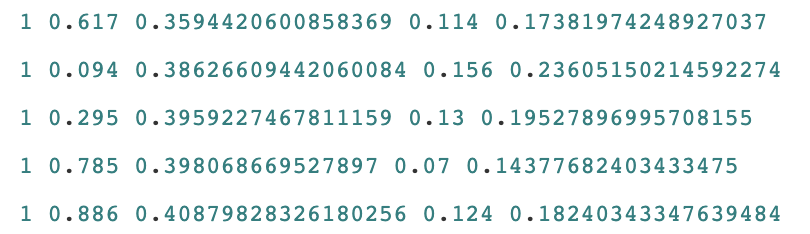
\includegraphics[scale=0.6]{img/formato_pvz.png}
    \caption{„YOLO PyTorch TXT“ formato nuotraukos objektų failas.}
    \label{img:format}
\end{figure}

„Amazon Rekognition“ grąžina aptiktų objektų stačiakampių koordinates kitokiu formatu negu reikalauja YOLO modelis, todėl privaloma jas konvertuoti. Pasitelkiant „roboflow“ programa, tai atliekama automatiškai - pateikus failą su visų nuotraukoje aptiktų objektų koordinatėmis ir aptiktu objektu, jis automatiškai konvertuoja jas į pasirinktą formatą, šiuo atveju „YOLO PyTorch TXT“.

\subsubsection{Nuotraukų augmentacija}
Nuotraukų augmentacija, arba duomenų augmentacija yra technika, naudojama mašininiame mokyme, kad padidinti mokymosi duomenų rinkinio dydį. Tai yra įgyvendinama kuriant modifikuotas duomenų rinkinio nuotraukas. Modifikavimas apima veiksmus, tokius kaip nuotraukų pasukimas, apvertimas, apkarpymas, triukšmo (angl. \emph{noise}) pridėjimas, ar atspalvių keitimas. Augmentacijos tikslas yra apsisaugoti nuo persimokymo \cite{perez2017effectiveness}, kuris atsiranda, kai modelis gerai veikia su mokymosi duomenimis, bet prastai su nematytais duomenimis. 

Šiam duomenų rinkiniui buvo pritaikytos 4 augmentacijos - nuotraukos apkarpymas, pasukimas, šviesumo pakeitimas ir triukšmo pridėjimas. Šviesumo pakeitimas ir triukšmo pridėjimas pasirinktas dėl to, kad gilaus mokymo modelis galėtų tinkamai atpažinti objektus kai jų vaizdas pasikeičia dėl aplinkos sąlygų, pavyzdžiui, apšvietimo ar oro sąlygų \cite{MUMUNI2022100258}. Nuotraukos apkarpymas ir pasukimas buvo pasirinktas, nes yra ne tik paprastas būdas praplėsti duomenų rinkinį, bet ir labai efektyvus daugumoje kompiuterinės regos užduočių. \cite{xu2016improved}. Taip pat YOLO objektų atpažinimo modelis reikalauja duomenų rinkinio su vienodu nuotraukų dydžiu. Šiame darbe jis buvo pasirinktas 640 x 640 pikselių. Nuotraukų augmentacijos pavyzdys pateiktas \ref{img:mergedaug} pav.

\begin{figure}[H]
    \centering
    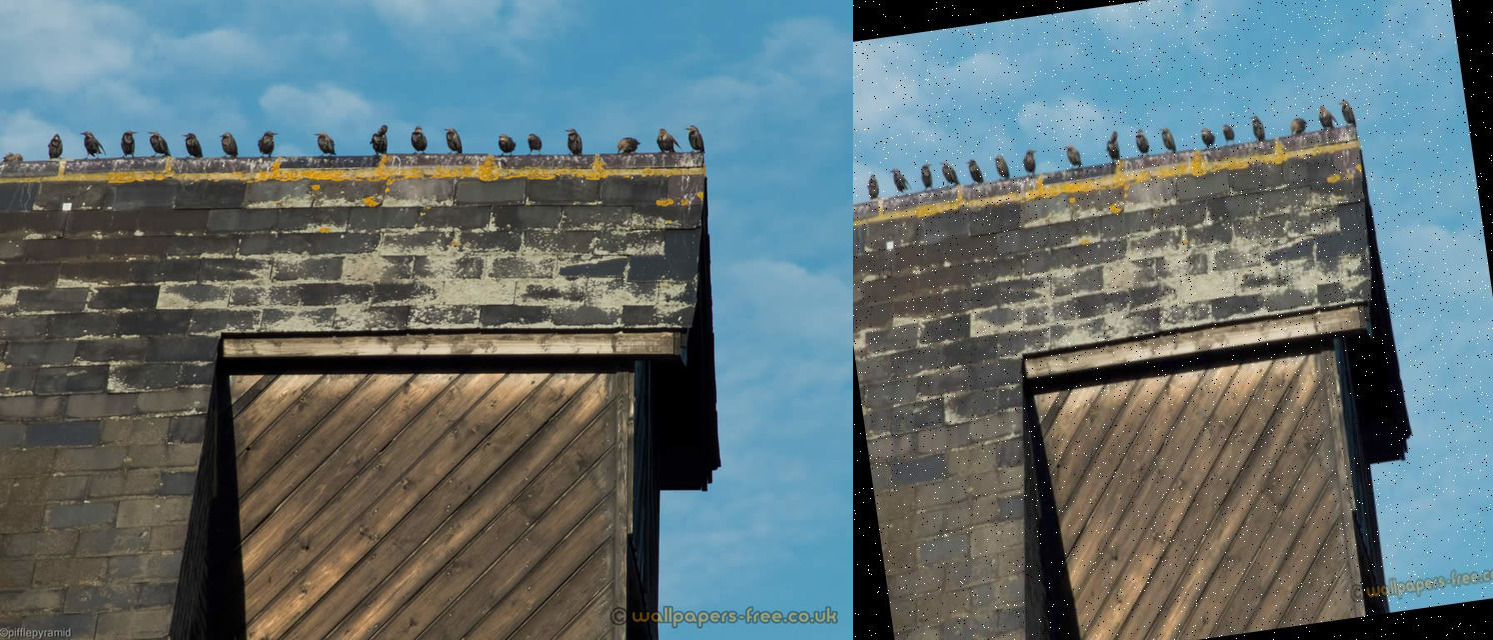
\includegraphics[width=1\textwidth]{img/imgformat.jpg}
    \caption{Nuotrauka prieš augmentaciją (kairėje) ir po (dešinėje).}
    \label{img:mergedaug}
\end{figure}

\subsubsection{Duomenų rinkinio eksportavimas iš „roboflow“}
Pabaigus konfigūruoti rinkinį ir jį augmentuoti reikalingas eksportavimas, kad būtų galima pradėti mokymą su juo. Nors ir yra galimybė apmokinti objektų aptikimo modelį pačiame „roboflow“ - tai nėra geras būdas šiam sprendimui. Pasirinkus mokymą jų sistemoje negalima keisti jokių hiperparametrų, bei objektų aptikimo modelių. Tai būtų naudinga jei norima būtų lyginti tik duomenų rinkinius, tačiau šiuo atveju tai nėra geras sprendimas ir dėl to, kad negalima parsisiųsti pačio modelio - galima tik vykdyti išvadų darymą (angl. \emph{inference}) per jų sąsają ar per patį internetinį tinklapį. Šiam sprendimui reikalinga vykdyti išvadų darymą pačiame įrenginyje, kad atbaidymas vyktų greičiau.

Išeksportavus duomenų rinkinį tinkamu formatu, šiuo atveju „YOLO PyTorch TXT” gauname suarchyvuotą failą su visomis rinkinio treniravimo, validavimo ir treniravimo nuotraukomis, tų nuotraukų aptiktų objektų anotacijomis ir „YAML“ (angl. \emph{„Yet Another Markup Language“}) formatu pateikta YOLO konfiguracija. Išarchyvuoto failo pavyzdys pateiktas \ref{img:config_dataset.png} pav.

\begin{figure}[H]
    \centering
    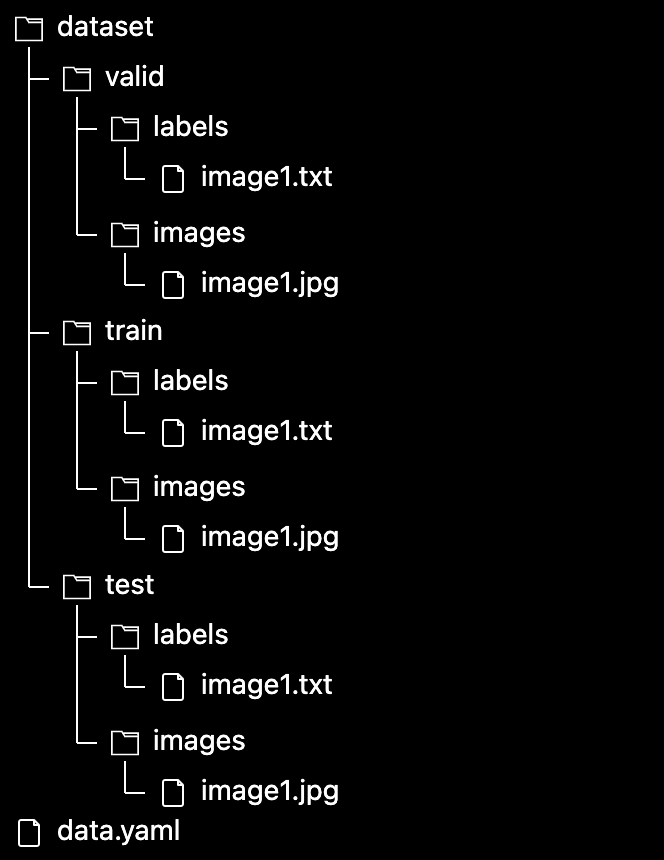
\includegraphics[scale=0.6]{img/config_dataset.png}
    \caption{YOLO formato duomenų rinkinio pavyzdys.}
    \label{img:config_dataset.png}
\end{figure}

\section{Objektų aptikimo modeliai}
Giliojo mokymosi objektų aptikimo modeliai galima skirstyti į dvi kategorijas: dviejų etapų, tokie kaip R-CNN, Faster R-CNN ir vieno etapo, YOLO, SSD ar RetinaNet \cite{jiao2019survey}. Dviejų etapų objektų atpažinimo modeliai turi didesnį lokalizavimo ir objektų aptikimo tikslumą, tuo tarpu vieno etapo geba greičiau daryti išvadas. Šiame darbe buvo pasirinkta naudoti YOLO modelį kadangi lyginant visų modelių greitį ir tikslumą aptikti objektus, buvo pastebėta, kad tam tikros YOLO versijos tai atlieka greičiau ir tiksliau \cite{wang2022yolov7}. Palyginimui buvo paimtos trys skirtingos YOLO versijos: YOLOv5 \cite{Jocher_YOLOv5_by_Ultralytics_2020}, YOLOv7 ir YOLOv8 \cite{Jocher_YOLO_by_Ultralytics_2023}. 

\subsection{YOLO algoritmas}
YOLO algoritmas buvo sukurtas, kad galėtų atlikti atpažinti objektus per vieną algoritmo paleidimą, todėl ir vadinasi You Only Look Once. Vietoj ieškojimo regionų, kurie turėtų norimą objektą, YOLO naudoja visą nuotrauką ir ją padalina į $S$ x $S$ ląstelių ir jeigu objekto centras pakliūna į ląstelę, ji tampa atsakinga už to objekto aptikimą. Kiekvienas toks kvadratas yra atsakingas spėjant B kiekį objektą apibrėžiančių stačiakampių ir skaičių, kaip užtikrintai jis spėja aptikto objekto ribas ir patį objektą \cite{redmon2015you}. Veikimo pavyzdys pateiktas \ref{img:yoloalg.png} pav. 

\begin{figure}[H]
    \centering
    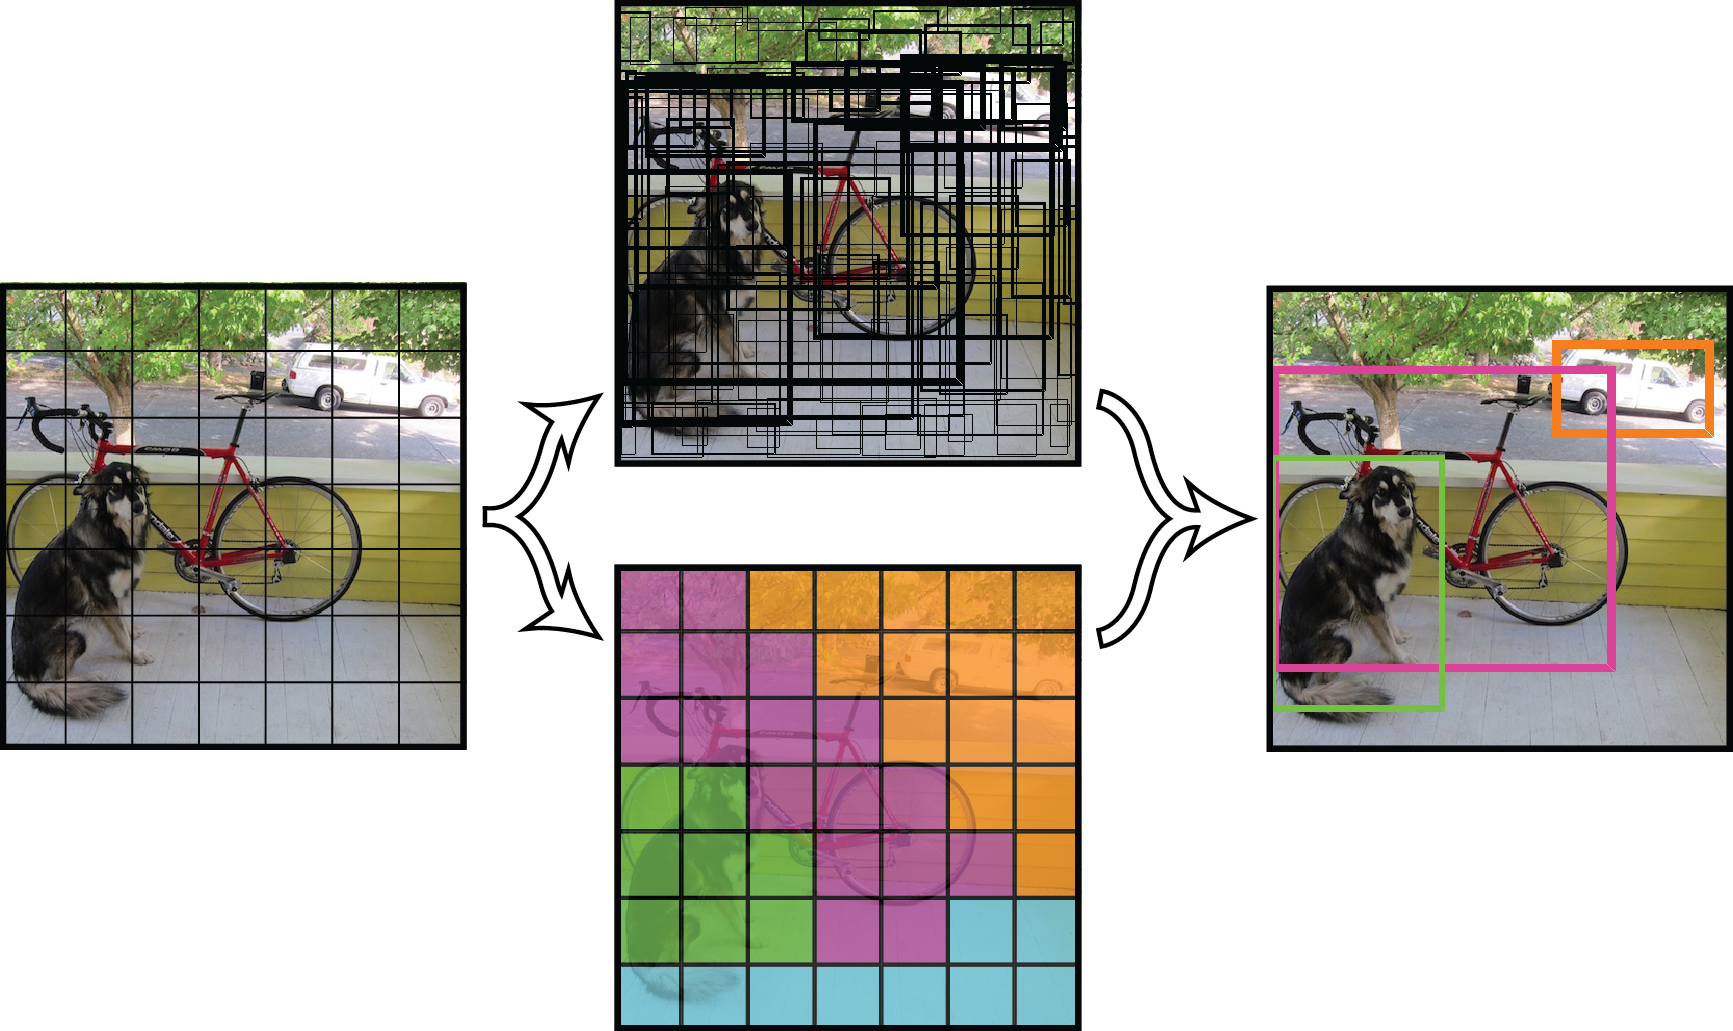
\includegraphics[width=1\textwidth]{img/yolo_algo.png}
    \caption{YOLO algoritmo pavyzdys. Šaltinis: \cite{redmon2015you}}
    \label{img:yoloalg.png}
\end{figure}

Kiekvienas stačiakampis susidaro iš penkių parametrų: $x, y, w, h$ ir pasitikėjimas (angl. \emph{confidence}). $x$ ir $y$ koordinatės nurodo centrą spėto apibrėžiančio stačiakampio kvadrato kraštų atžvilgiu. $w$ ir $h$ rodo stačiakampio plotį ir aukštį visos nuotraukos dydžio atžvilgiu. Pasitikėjimas rodo tikrumą dėl klasės ir apibrėžiančio stačiakampio koordinačių. YOLO tinklas kiekvienam kvadratui, iš kurių susideda pilna nuotraukas, išveda $S$ x $S$ x $(5B + C)$ tenzorių, kur $C$ - spėjamų klasių kiekis, $B$ - spėjimų kiekis vienam kvadratui. Pavydžiui, pasirinkus $S = 7, B = 2$ ir $C = 20$ gausime, kad tenzorių $7 × 7 × 30$.

\subsection{Modelių mokymas}
Visų modelių mokymas ir testavimas buvo vykdomas „Google Colab“ aplinkoje, naudojant nemokamą versiją. Vaizdo plokštė naudojama buvo Nvidia Tesla T4. Kiekvienas modelis buvo mokomas 50 epochų.  Pradinis mokymosi greitis buvo 0.01, tačiau jis buvo keičiamas naudojant kosinuso atkaitinimo algoritmą (angl. \emph{Cosine Annealing}). Visi modeliai buvo mokyti naudojant svorius iš COCO duomenų rinkinio.

\subsubsection{1 modelis: YOLOv5}
YOLOv5 buvo išleistas 2020, kaip YOLOv3 tesinys, tačiau perdarytas naudojant PyTorch karkasą, vietoj Darknet. Modelis susideda iš trijų dalių: stuburo (angl. \emph{backbone}) tinklo, kaklo (angl. \emph{neck}) tinklo ir galvos (angl. \emph{head}) tinklo. Stuburo tinklas naudoja CSP-Darknet53, jis naudoja SPP(Spatial Pyramid Pooling), kad išgautų požymius \cite{DBLP:journals/corr/abs-1911-11929}. Kaklas naudoja PA-Net, kad surinktų požymius iš kaklo tinklo skirtingų sluoksnių \cite{panet}. Galva naudoja YOLOv4, kuri spėja apibrėžiančio stačiakampio koordinates, aptiktą objektą ir pasitikėjimą.

\subsubsection{2 modelis: YOLOv7}
YOLOv7 buvo išleistas 2022. Išleidimo metu tai buvo efektyviausias modelis, kuris buvo sukurtas tobulinant Scaled YOLOv4\cite{scaledyolov4}. Šis modelis vietoje CSP-Darknet53, kuris yra naudojamas YOLOv5, naudoja E-ELAN tinklą \cite{wang2022yolov7}. Taip pat, YOLOv7 turi daugiau nei vieną galvą. Galva, kuri yra atsakinga už galutinį spėjimą yra pagrindė galva, o kita galva, vadinama pagalbinė galva, naudojama pagelbėti mokymuisi.

\subsubsection{3 modelis: YOLOv8}
YOLOv8 buvo išleistas 2023. Tai yra naujausias YOLO šeimos modelių versija. Kadangi modelis yra naujai išleistas, dar nėra parašytas jo mokslinis darbas, dėl to jo architektūrą yra sunku palyginti su kitomis. 

\subsection{Modelių vertinimas}
Dažnai naudojama metrika palyginti objektų aptikimo veiksmingumą yra suvidurkintas aptikimo tikslumas (angl. \emph{mean Average Precision}, mAP) \cite{meanaverage}. Apskaičiuojant suvidurkintą aptikimo tikslumą yra naudojamas aptikto objekto ir tikrų jo ribų (angl. \emph{ground truth}) stačiakampių sankirtos ir sąjungos santykis (angl. \emph{intersection over union}, IOU) dydis. Šiuo dydžių siekiama, kad spėjamas stačiakampis būtų kuo panašesnis į tikrą stačiakampį (tokiu atveju IOU dydis būtų 1). Kuo mažesnis šis dydis, tuo labiau skiriasi spėtas stačiakampis nuo tikrojo ir tikslumas būna jo mažesnis. Standartiškai laikoma, kad jeigu sankirtos ir sąjungos santykis yra didesnis negu 50 \% arba 0,5 tada spėjimas yra teisingas. Taip pat, skaičiuojant suvidurkintą aptikimo tikslumą reikia apskaičiuoti kiek objektų buvo atpažinti teisingai (angl. \emph{true positive}, TP), neteisingai (angl. \emph{false positive}, FP) ir neatpažinta (angl. \emph{False negative}, FN). Spėjimas būna teisingas, jeigu jis teisingai atspėja klasę ir jo sankirtos ir sąjungos santykis būna didesnis negu nustatyta riba. Spėjimas būna neteisingas, jeigu bent viena prieš tai minėta sąlyga nebūna įvykdyta. Turint šiuos skaičius galima skaičiuoti klasės tikslumą (angl. \emph{precision}) ir jautrumą (angl. \emph{recall}). Turint šiuos skaičius ir išvedę vidurkį iš visų klasių gauname vidutinį suvidurkintą tikslumą (angl. \emph{mean Average Precision}, mAP).

\subsection{Modelių palyginimas}
Atlikus visų modelių mokymą su savarankiškai surinktu duomenų rinkiniu, galime matyti jų skirtumus \ref{tab:my-table} lentelėje. Kaip matome, seniausiai kurtas modelis YOLOv5 atsilieka nuo YOLOv7 ir YOLOv8. 
Jis yra paskutinis visose kategorijose išskyrus mokymosi trukmę. Tai rodo, kad naujesni modėliai yra pasimokę iš senų klaidų ir jas patobulinę. Įdomu, kad jo jautrumas yra 0,48, o tai rodo, kad jis labiau linkęs neaptikti nieko, negu aptikti klaidingai.  Vidutinis suvidurkintas tikslumas jo yra 58 \%, o tai yra 27,5 \% mažiau negu geriausią rezultatą turinčio modelio - YOLOv7.

YOLOv7 turi geriausius mAP, tikslumo ir jautrumo rezultatus, tačiau jo mokymosi laikas yra 41 \% didesnis negu trumpiausią laiką turinčio modelio. Taip pat jo spėjimo greitis atsilieka 0,8 sekundėmis nuo geriausio laiko. 

YOLOv8 turi antrą geriausią mAP, tikslumą ir jautrumą. Jis pirmauja pagal spėjimo greitį ir mokymosi trukmę. Šį modelį kol kas sunku lyginti su senesniais modeliais, nes jis yra labai naujas (Išleistas sausio 10d.) ir neturi tokios brandos, kokias turi prieštai minėti modeliai. 

Paukščių aptikimo ir atbaidymo užduotis reikalauja aukšto tikslumo ir greito reagavimo, dėl šitų reikalavimų geriausia būtų rinktis YOLOv7 modelį, kadangi jo mAP yra 80 \% ir spėjimo greitis neatsilieka tiek daug, kad sukeltų didelių bėdų atbaidant.

\begin{table}[H]
\centering
\resizebox{\textwidth}{!}{%
\begin{tabular}{|l|c|c|c|c|c|}
\hline
Modelis &
  \multicolumn{1}{l|}{mAP (\%)} &
  \multicolumn{1}{l|}{Tikslumas} &
  \multicolumn{1}{l|}{Jautrumas} &
  \multicolumn{1}{l|}{Spėjimo greitis  (milisekundėmis)} &
  \multicolumn{1}{l|}{Mokymosi trukmė (minutėmis)} \\ \hline
YOLOv5 & 58,0 & 0,71 & 0,48 & 14,8 & 20,82 \\ \hline
YOLOv7 & 80,5 & 0,77 & 0,75 & 14,4 & 34,38 \\ \hline
YOLOv8 & 73,6 & 0,72 & 0,68 & 13,6 & 19,86 \\ \hline
\end{tabular}%
}
\caption{YOLO modelių rezultatai.}
\label{tab:my-table}
\end{table}


\section{Siūlomas sprendimas paukščių atbaidymui}
Paukščių aptikimo ir atbaidymo sprendimas turėtų susidėti iš šių komponentų:
\begin{enumerate}
    \item PTZ kameros
    \item Žalio lazerio
    \item Lazerio laikiklio gebančio pasisukti ir pasikreipti
    \item Paukščius aptikti gebančio modelio
    \item Algoritmo gebančio apskaičiuoti lazerio švietimo krypti pagal aptiktų paukščių koordinates
    \item Mini kompiuterio
\end{enumerate}

Turint šiuos komponentus, būtų galima įgyvendinti paukščių aptikimo ir atbaidymo sprendimą. Šį sprendimą, būtų galima statyti miestuose, kad humaniškai apsaugoti turtą nuo paukščių.
\subsection{Saugumas}
Naudojant lazerius dažnai reikia laikytis saugumo priemonių. Kadangi ši sistema yra paremta dirbtiniu intelektu, ji kartais gali padaryti klaidų. Taip pat \ref{tab:my-table} lentelėje matėme, kad visi modeliai turi didesni negu 0,48 jautrumą, o tai reiškia, kad jie gali suveikti net jeigu nėra visiškai tikri ar ten teisingai aptiktas objektas. Todėl yra keletas siūlymų, kaip būtų galima apsisaugoti nuo tokių klaidų:

\begin{enumerate}
    \item Nubrėžiamos ribos - sistema gebėtų priimti ribas, kuriuose turėtų ieškoti paukščių ir veikti tik nubrėžtose ribose. Taip būtų galima apibrėžti stogą ir visas veikimas vyktų tik jo teritorijoje.
    \item Tobulinamas modelis - jeigu modelis gebėtų tobulai klasifikuoti objektus, tada jis taptų saugesnis, nes pašaliniai objektai nebūtų atpažinti kaip paukščiai ir nebūtų šviečiamas lazeris į juos.
    \item Tobulinamas duomenų rinkinys - reikalingas, kad tobulinant modelį jis galėtų geriau generalizuoti duomenis ir būtų tikresnis dėl aptiktų objektų.
\end{enumerate}

\subsection{Ateities darbai}
Tęsiant šį darbą reikėtų surinkti didesnį ir įvairesnį duomenų rinkinį. Tinkamiausias būdas būtų palikti stebėjimo kamerą mieste, kur renkasi paukščių būriai. Norint, kad sprendimas veiktų kuo geriau ir būtų pritaikomas plačiau, reikėtų daugiau tokių vietų, kad susidarytų kuo įvairesnis duomenų rinkinys. Taip pat, reikėtų sukurti sprendimą, kuris gebėtų iš nuotraukoje aptiktų objektų koordinačių, šviesti lazerį į tą vietą.


\sectionnonum{Rezultatai ir išvados}
Šiame darbe buvo apžvelgti skirtingi paukščių atbaidymo būdai, bei surastas tinkamiausias giliojo mokymosi modelis gebantis atpažinti ir lokalizuoti paukščius esančius miesto erdvėse - YOLOv7. Jis pasiekė 80,5 \% suvidurkintą aptikimo tikslumą per gana nedidelį laiką - 14,4 milisekundes. Tai rodo, kad jis yra tinkamas modelis naudoti paukščių atpažinimo uždaviniams spręsti, tačiau yra būdų dar kaip jį tobulinti. Taip pat pastebėta, kad norint paleistį tokį sprendimą gyvai, reikėtų įdiegti papildomas saugumo priemones. Darbo išvados:
\begin{enumerate}
    \item Geriausią rezultatą rodantis modelis yra YOLOv7.
    \item Reikalingas didesnis ir įvairesnis duomenų rinkinys norint saugiau įgyvendinti paukščių aptikimą ir atbaidymą.
\end{enumerate}


\printbibliography[heading=bibintoc]  

\sectionnonum{Santrumpos}
\begin{itemize}
    \item YOLO - „You only look once“ objektų aptikimo algoritmas.
    \item mAP - suvidurkintas aptikimo tikslumas (angl. \emph{mean Average Precision})
    \item BBID - angl. \emph{Bulk Bing Image Downloader}
    \item PTZ - pasvirimas, pakreipimas, priartinimas (angl. \emph{pan, tilt, zoom})
\end{itemize}

\end{document}
